% Options for packages loaded elsewhere
\PassOptionsToPackage{unicode}{hyperref}
\PassOptionsToPackage{hyphens}{url}
\PassOptionsToPackage{dvipsnames,svgnames,x11names}{xcolor}
%
\documentclass[
  letterpaper,
  DIV=11,
  numbers=noendperiod,
  oneside]{scrreprt}

\usepackage{amsmath,amssymb}
\usepackage{lmodern}
\usepackage{iftex}
\ifPDFTeX
  \usepackage[T1]{fontenc}
  \usepackage[utf8]{inputenc}
  \usepackage{textcomp} % provide euro and other symbols
\else % if luatex or xetex
  \usepackage{unicode-math}
  \defaultfontfeatures{Scale=MatchLowercase}
  \defaultfontfeatures[\rmfamily]{Ligatures=TeX,Scale=1}
\fi
% Use upquote if available, for straight quotes in verbatim environments
\IfFileExists{upquote.sty}{\usepackage{upquote}}{}
\IfFileExists{microtype.sty}{% use microtype if available
  \usepackage[]{microtype}
  \UseMicrotypeSet[protrusion]{basicmath} % disable protrusion for tt fonts
}{}
\makeatletter
\@ifundefined{KOMAClassName}{% if non-KOMA class
  \IfFileExists{parskip.sty}{%
    \usepackage{parskip}
  }{% else
    \setlength{\parindent}{0pt}
    \setlength{\parskip}{6pt plus 2pt minus 1pt}}
}{% if KOMA class
  \KOMAoptions{parskip=half}}
\makeatother
\usepackage{xcolor}
\usepackage[left=1in,marginparwidth=2.0666666666667in,textwidth=4.1333333333333in,marginparsep=0.3in]{geometry}
\setlength{\emergencystretch}{3em} % prevent overfull lines
\setcounter{secnumdepth}{5}
% Make \paragraph and \subparagraph free-standing
\ifx\paragraph\undefined\else
  \let\oldparagraph\paragraph
  \renewcommand{\paragraph}[1]{\oldparagraph{#1}\mbox{}}
\fi
\ifx\subparagraph\undefined\else
  \let\oldsubparagraph\subparagraph
  \renewcommand{\subparagraph}[1]{\oldsubparagraph{#1}\mbox{}}
\fi

\usepackage{color}
\usepackage{fancyvrb}
\newcommand{\VerbBar}{|}
\newcommand{\VERB}{\Verb[commandchars=\\\{\}]}
\DefineVerbatimEnvironment{Highlighting}{Verbatim}{commandchars=\\\{\}}
% Add ',fontsize=\small' for more characters per line
\usepackage{framed}
\definecolor{shadecolor}{RGB}{241,243,245}
\newenvironment{Shaded}{\begin{snugshade}}{\end{snugshade}}
\newcommand{\AlertTok}[1]{\textcolor[rgb]{0.68,0.00,0.00}{#1}}
\newcommand{\AnnotationTok}[1]{\textcolor[rgb]{0.37,0.37,0.37}{#1}}
\newcommand{\AttributeTok}[1]{\textcolor[rgb]{0.40,0.45,0.13}{#1}}
\newcommand{\BaseNTok}[1]{\textcolor[rgb]{0.68,0.00,0.00}{#1}}
\newcommand{\BuiltInTok}[1]{\textcolor[rgb]{0.00,0.23,0.31}{#1}}
\newcommand{\CharTok}[1]{\textcolor[rgb]{0.13,0.47,0.30}{#1}}
\newcommand{\CommentTok}[1]{\textcolor[rgb]{0.37,0.37,0.37}{#1}}
\newcommand{\CommentVarTok}[1]{\textcolor[rgb]{0.37,0.37,0.37}{\textit{#1}}}
\newcommand{\ConstantTok}[1]{\textcolor[rgb]{0.56,0.35,0.01}{#1}}
\newcommand{\ControlFlowTok}[1]{\textcolor[rgb]{0.00,0.23,0.31}{#1}}
\newcommand{\DataTypeTok}[1]{\textcolor[rgb]{0.68,0.00,0.00}{#1}}
\newcommand{\DecValTok}[1]{\textcolor[rgb]{0.68,0.00,0.00}{#1}}
\newcommand{\DocumentationTok}[1]{\textcolor[rgb]{0.37,0.37,0.37}{\textit{#1}}}
\newcommand{\ErrorTok}[1]{\textcolor[rgb]{0.68,0.00,0.00}{#1}}
\newcommand{\ExtensionTok}[1]{\textcolor[rgb]{0.00,0.23,0.31}{#1}}
\newcommand{\FloatTok}[1]{\textcolor[rgb]{0.68,0.00,0.00}{#1}}
\newcommand{\FunctionTok}[1]{\textcolor[rgb]{0.28,0.35,0.67}{#1}}
\newcommand{\ImportTok}[1]{\textcolor[rgb]{0.00,0.46,0.62}{#1}}
\newcommand{\InformationTok}[1]{\textcolor[rgb]{0.37,0.37,0.37}{#1}}
\newcommand{\KeywordTok}[1]{\textcolor[rgb]{0.00,0.23,0.31}{#1}}
\newcommand{\NormalTok}[1]{\textcolor[rgb]{0.00,0.23,0.31}{#1}}
\newcommand{\OperatorTok}[1]{\textcolor[rgb]{0.37,0.37,0.37}{#1}}
\newcommand{\OtherTok}[1]{\textcolor[rgb]{0.00,0.23,0.31}{#1}}
\newcommand{\PreprocessorTok}[1]{\textcolor[rgb]{0.68,0.00,0.00}{#1}}
\newcommand{\RegionMarkerTok}[1]{\textcolor[rgb]{0.00,0.23,0.31}{#1}}
\newcommand{\SpecialCharTok}[1]{\textcolor[rgb]{0.37,0.37,0.37}{#1}}
\newcommand{\SpecialStringTok}[1]{\textcolor[rgb]{0.13,0.47,0.30}{#1}}
\newcommand{\StringTok}[1]{\textcolor[rgb]{0.13,0.47,0.30}{#1}}
\newcommand{\VariableTok}[1]{\textcolor[rgb]{0.07,0.07,0.07}{#1}}
\newcommand{\VerbatimStringTok}[1]{\textcolor[rgb]{0.13,0.47,0.30}{#1}}
\newcommand{\WarningTok}[1]{\textcolor[rgb]{0.37,0.37,0.37}{\textit{#1}}}

\providecommand{\tightlist}{%
  \setlength{\itemsep}{0pt}\setlength{\parskip}{0pt}}\usepackage{longtable,booktabs,array}
\usepackage{calc} % for calculating minipage widths
% Correct order of tables after \paragraph or \subparagraph
\usepackage{etoolbox}
\makeatletter
\patchcmd\longtable{\par}{\if@noskipsec\mbox{}\fi\par}{}{}
\makeatother
% Allow footnotes in longtable head/foot
\IfFileExists{footnotehyper.sty}{\usepackage{footnotehyper}}{\usepackage{footnote}}
\makesavenoteenv{longtable}
\usepackage{graphicx}
\makeatletter
\def\maxwidth{\ifdim\Gin@nat@width>\linewidth\linewidth\else\Gin@nat@width\fi}
\def\maxheight{\ifdim\Gin@nat@height>\textheight\textheight\else\Gin@nat@height\fi}
\makeatother
% Scale images if necessary, so that they will not overflow the page
% margins by default, and it is still possible to overwrite the defaults
% using explicit options in \includegraphics[width, height, ...]{}
\setkeys{Gin}{width=\maxwidth,height=\maxheight,keepaspectratio}
% Set default figure placement to htbp
\makeatletter
\def\fps@figure{htbp}
\makeatother
\newlength{\cslhangindent}
\setlength{\cslhangindent}{1.5em}
\newlength{\csllabelwidth}
\setlength{\csllabelwidth}{3em}
\newlength{\cslentryspacingunit} % times entry-spacing
\setlength{\cslentryspacingunit}{\parskip}
\newenvironment{CSLReferences}[2] % #1 hanging-ident, #2 entry spacing
 {% don't indent paragraphs
  \setlength{\parindent}{0pt}
  % turn on hanging indent if param 1 is 1
  \ifodd #1
  \let\oldpar\par
  \def\par{\hangindent=\cslhangindent\oldpar}
  \fi
  % set entry spacing
  \setlength{\parskip}{#2\cslentryspacingunit}
 }%
 {}
\usepackage{calc}
\newcommand{\CSLBlock}[1]{#1\hfill\break}
\newcommand{\CSLLeftMargin}[1]{\parbox[t]{\csllabelwidth}{#1}}
\newcommand{\CSLRightInline}[1]{\parbox[t]{\linewidth - \csllabelwidth}{#1}\break}
\newcommand{\CSLIndent}[1]{\hspace{\cslhangindent}#1}

\usepackage{booktabs}
\usepackage{longtable}
\usepackage{array}
\usepackage{multirow}
\usepackage{wrapfig}
\usepackage{float}
\usepackage{colortbl}
\usepackage{pdflscape}
\usepackage{tabu}
\usepackage{threeparttable}
\usepackage{threeparttablex}
\usepackage[normalem]{ulem}
\usepackage{makecell}
\usepackage{xcolor}
\KOMAoption{captions}{tableheading}
\makeatletter
\@ifpackageloaded{tcolorbox}{}{\usepackage[many]{tcolorbox}}
\@ifpackageloaded{fontawesome5}{}{\usepackage{fontawesome5}}
\definecolor{quarto-callout-color}{HTML}{909090}
\definecolor{quarto-callout-note-color}{HTML}{0758E5}
\definecolor{quarto-callout-important-color}{HTML}{CC1914}
\definecolor{quarto-callout-warning-color}{HTML}{EB9113}
\definecolor{quarto-callout-tip-color}{HTML}{00A047}
\definecolor{quarto-callout-caution-color}{HTML}{FC5300}
\definecolor{quarto-callout-color-frame}{HTML}{acacac}
\definecolor{quarto-callout-note-color-frame}{HTML}{4582ec}
\definecolor{quarto-callout-important-color-frame}{HTML}{d9534f}
\definecolor{quarto-callout-warning-color-frame}{HTML}{f0ad4e}
\definecolor{quarto-callout-tip-color-frame}{HTML}{02b875}
\definecolor{quarto-callout-caution-color-frame}{HTML}{fd7e14}
\makeatother
\makeatletter
\makeatother
\makeatletter
\@ifpackageloaded{bookmark}{}{\usepackage{bookmark}}
\makeatother
\makeatletter
\@ifpackageloaded{caption}{}{\usepackage{caption}}
\AtBeginDocument{%
\ifdefined\contentsname
  \renewcommand*\contentsname{Table of contents}
\else
  \newcommand\contentsname{Table of contents}
\fi
\ifdefined\listfigurename
  \renewcommand*\listfigurename{List of Figures}
\else
  \newcommand\listfigurename{List of Figures}
\fi
\ifdefined\listtablename
  \renewcommand*\listtablename{List of Tables}
\else
  \newcommand\listtablename{List of Tables}
\fi
\ifdefined\figurename
  \renewcommand*\figurename{Figure}
\else
  \newcommand\figurename{Figure}
\fi
\ifdefined\tablename
  \renewcommand*\tablename{Table}
\else
  \newcommand\tablename{Table}
\fi
}
\@ifpackageloaded{float}{}{\usepackage{float}}
\floatstyle{ruled}
\@ifundefined{c@chapter}{\newfloat{codelisting}{h}{lop}}{\newfloat{codelisting}{h}{lop}[chapter]}
\floatname{codelisting}{Listing}
\newcommand*\listoflistings{\listof{codelisting}{List of Listings}}
\makeatother
\makeatletter
\@ifpackageloaded{caption}{}{\usepackage{caption}}
\@ifpackageloaded{subcaption}{}{\usepackage{subcaption}}
\makeatother
\makeatletter
\@ifpackageloaded{tcolorbox}{}{\usepackage[many]{tcolorbox}}
\makeatother
\makeatletter
\@ifundefined{shadecolor}{\definecolor{shadecolor}{rgb}{.97, .97, .97}}
\makeatother
\makeatletter
\@ifpackageloaded{sidenotes}{}{\usepackage{sidenotes}}
\@ifpackageloaded{marginnote}{}{\usepackage{marginnote}}
\makeatother
\makeatletter
\makeatother
\ifLuaTeX
  \usepackage{selnolig}  % disable illegal ligatures
\fi
\IfFileExists{bookmark.sty}{\usepackage{bookmark}}{\usepackage{hyperref}}
\IfFileExists{xurl.sty}{\usepackage{xurl}}{} % add URL line breaks if available
\urlstyle{same} % disable monospaced font for URLs
\hypersetup{
  pdftitle={fm-ggp2},
  pdfauthor={Martin Frigaard},
  colorlinks=true,
  linkcolor={blue},
  filecolor={Maroon},
  citecolor={Blue},
  urlcolor={Blue},
  pdfcreator={LaTeX via pandoc}}

\title{fm-ggp2}
\author{Martin Frigaard}
\date{1/6/2023}

\begin{document}
\maketitle
\ifdefined\Shaded\renewenvironment{Shaded}{\begin{tcolorbox}[boxrule=0pt, sharp corners, interior hidden, breakable, borderline west={3pt}{0pt}{shadecolor}, frame hidden, enhanced]}{\end{tcolorbox}}\fi

\renewcommand*\contentsname{Table of contents}
{
\hypersetup{linkcolor=}
\setcounter{tocdepth}{2}
\tableofcontents
}
\bookmarksetup{startatroot}

\hypertarget{preface}{%
\chapter*{Preface}\label{preface}}
\addcontentsline{toc}{chapter}{Preface}

Welcome! This website contains a collection of graphs created using
\texttt{ggplot2} (and friends!).

\begin{marginfigure}

{\centering 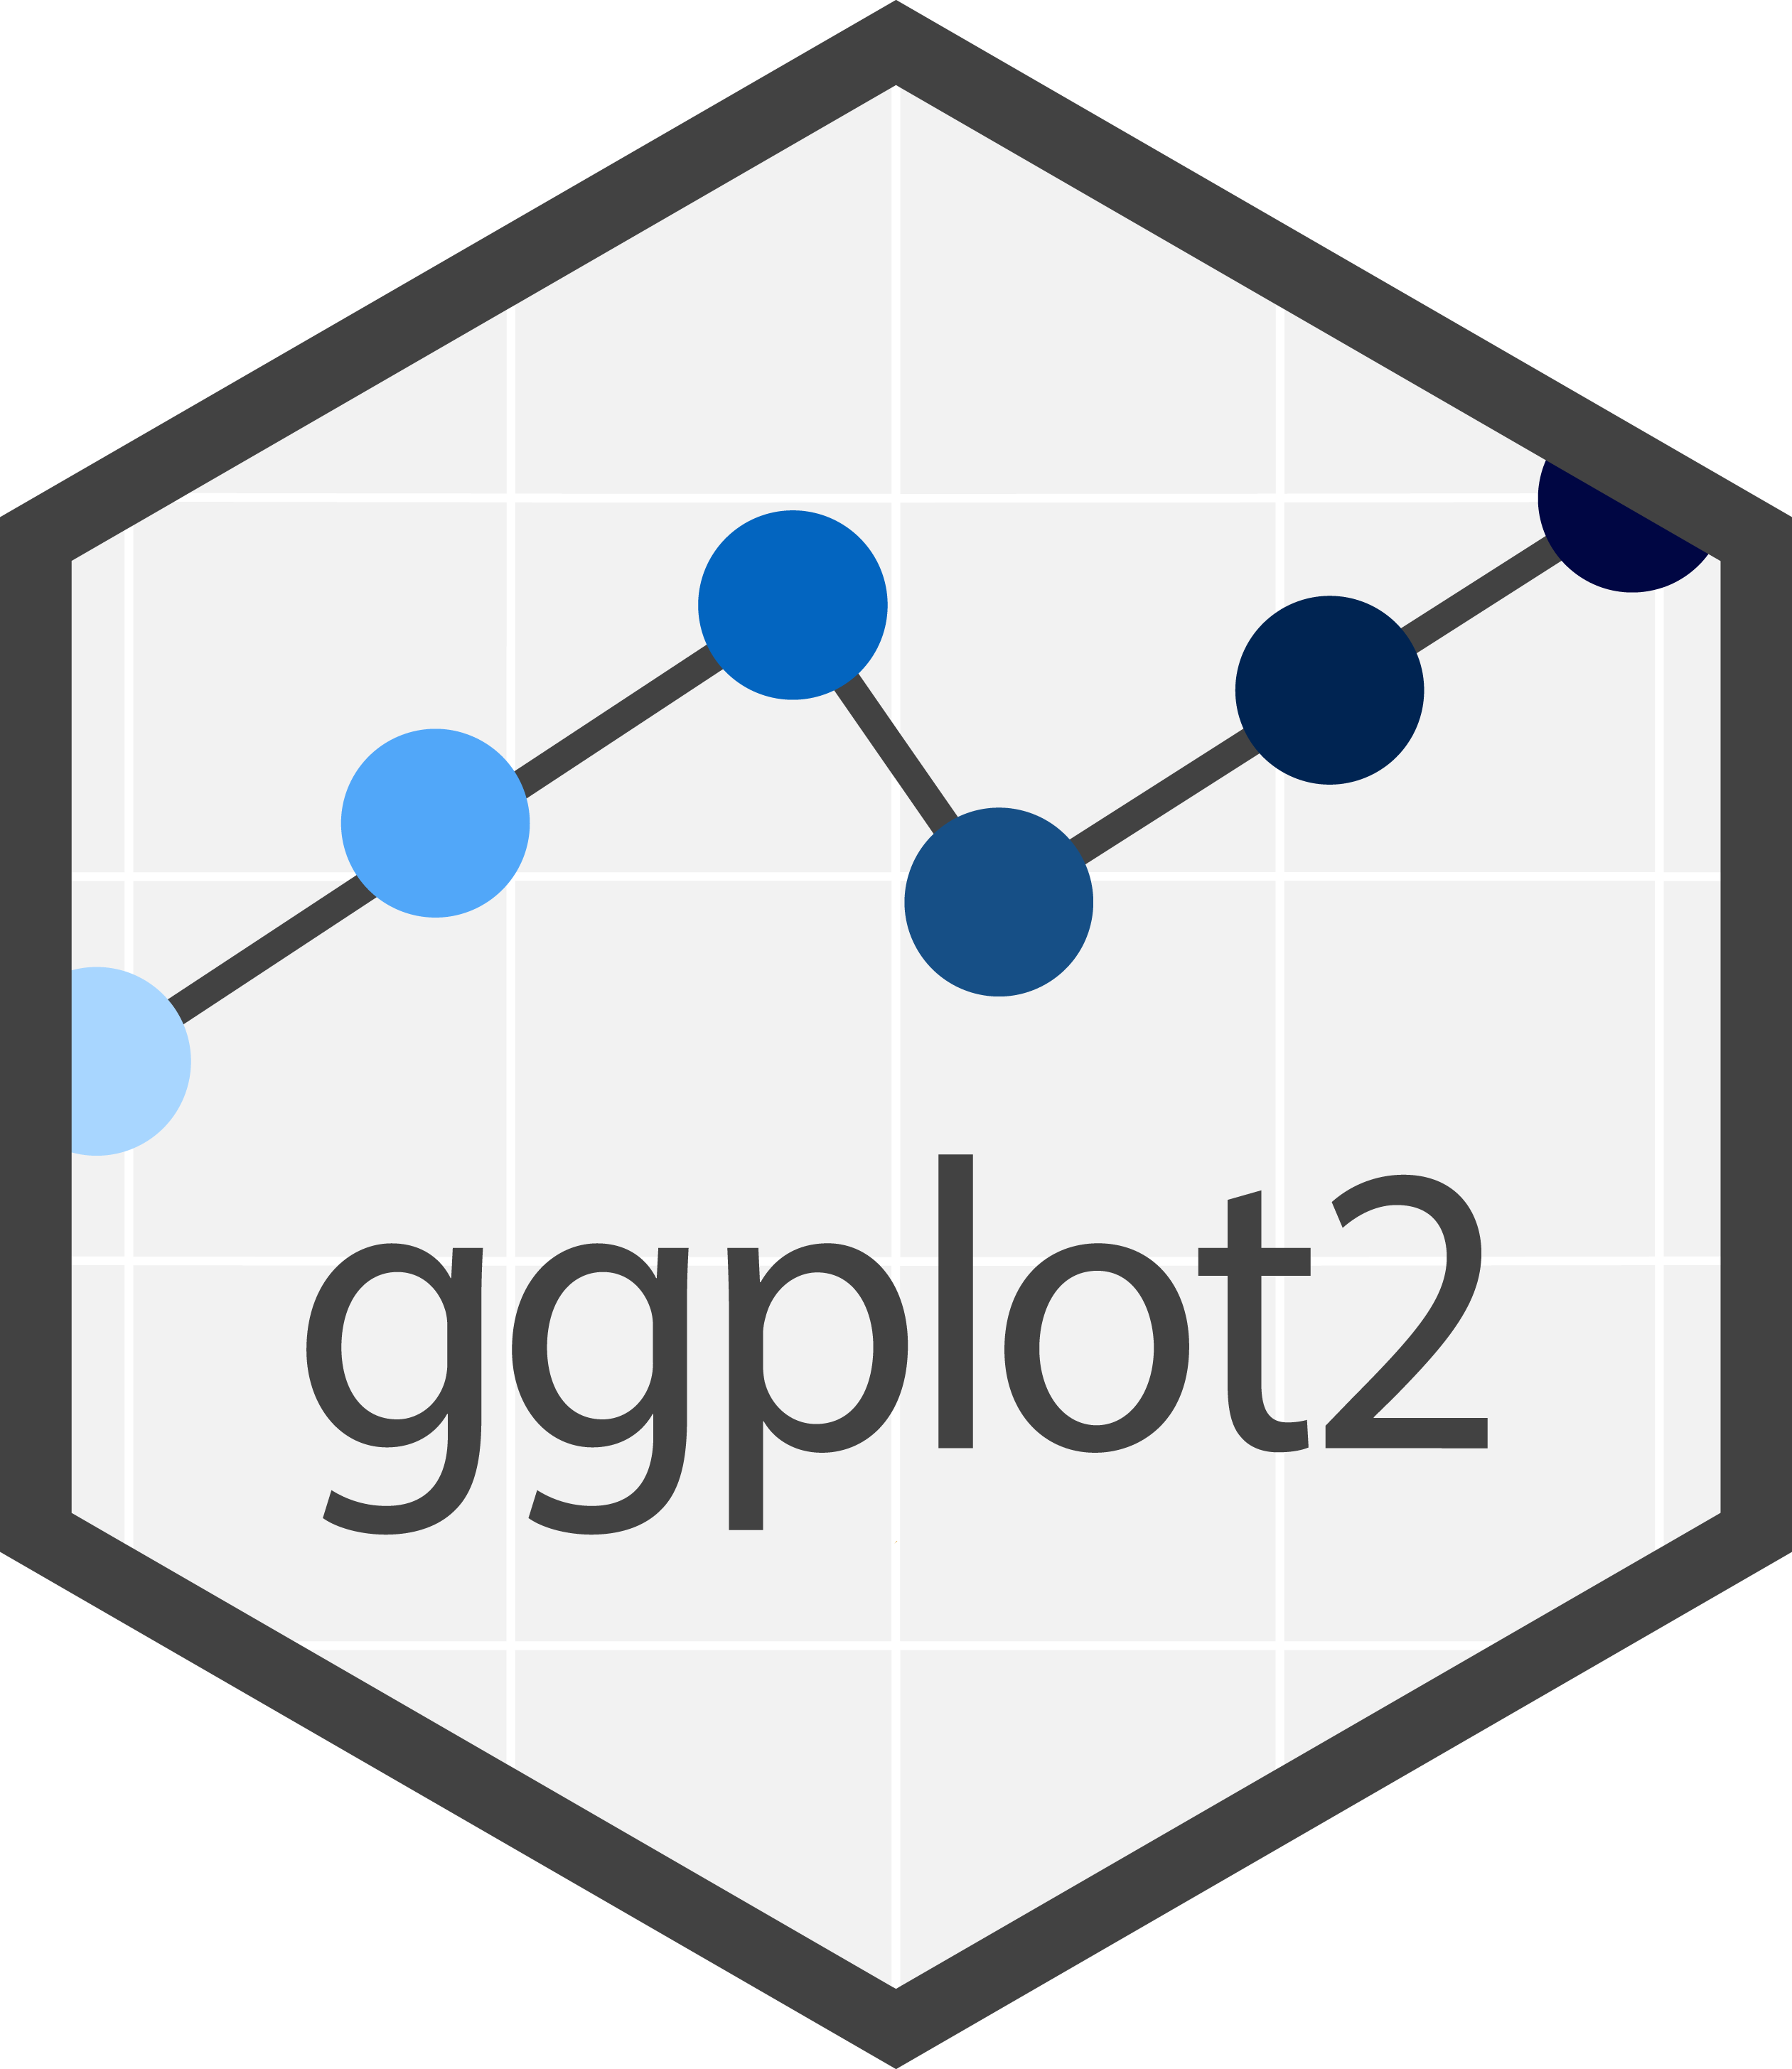
\includegraphics[width=0.4\textwidth,height=0.4\textheight]{./www/ggplot2.png}

}

\end{marginfigure}

Install \texttt{ggplot2} using the code below:

\begin{Shaded}
\begin{Highlighting}[]
\FunctionTok{install.packages}\NormalTok{(}\StringTok{"ggplot2"}\NormalTok{)}
\FunctionTok{library}\NormalTok{(ggplot2)}
\end{Highlighting}
\end{Shaded}

Or you can install \texttt{ggplot2} as part of the \texttt{tidyverse}:

\begin{marginfigure}

{\centering 
\includegraphics[width=0.4\textwidth,height=0.4\textheight]{./www/tidyverse.png}

}

\end{marginfigure}

\begin{Shaded}
\begin{Highlighting}[]
\FunctionTok{install.packages}\NormalTok{(}\StringTok{"tidyverse"}\NormalTok{)}
\FunctionTok{library}\NormalTok{(tidyverse)}
\end{Highlighting}
\end{Shaded}

\hypertarget{the-data}{%
\section*{The Data}\label{the-data}}
\addcontentsline{toc}{section}{The Data}

To improve reproducibility, the majority of the graphs are built using
the \texttt{palmerpenguins::penguins} data.

\textbf{\emph{\ldots so\ldots many\ldots PENGUINS!}}

\begin{marginfigure}

{\centering 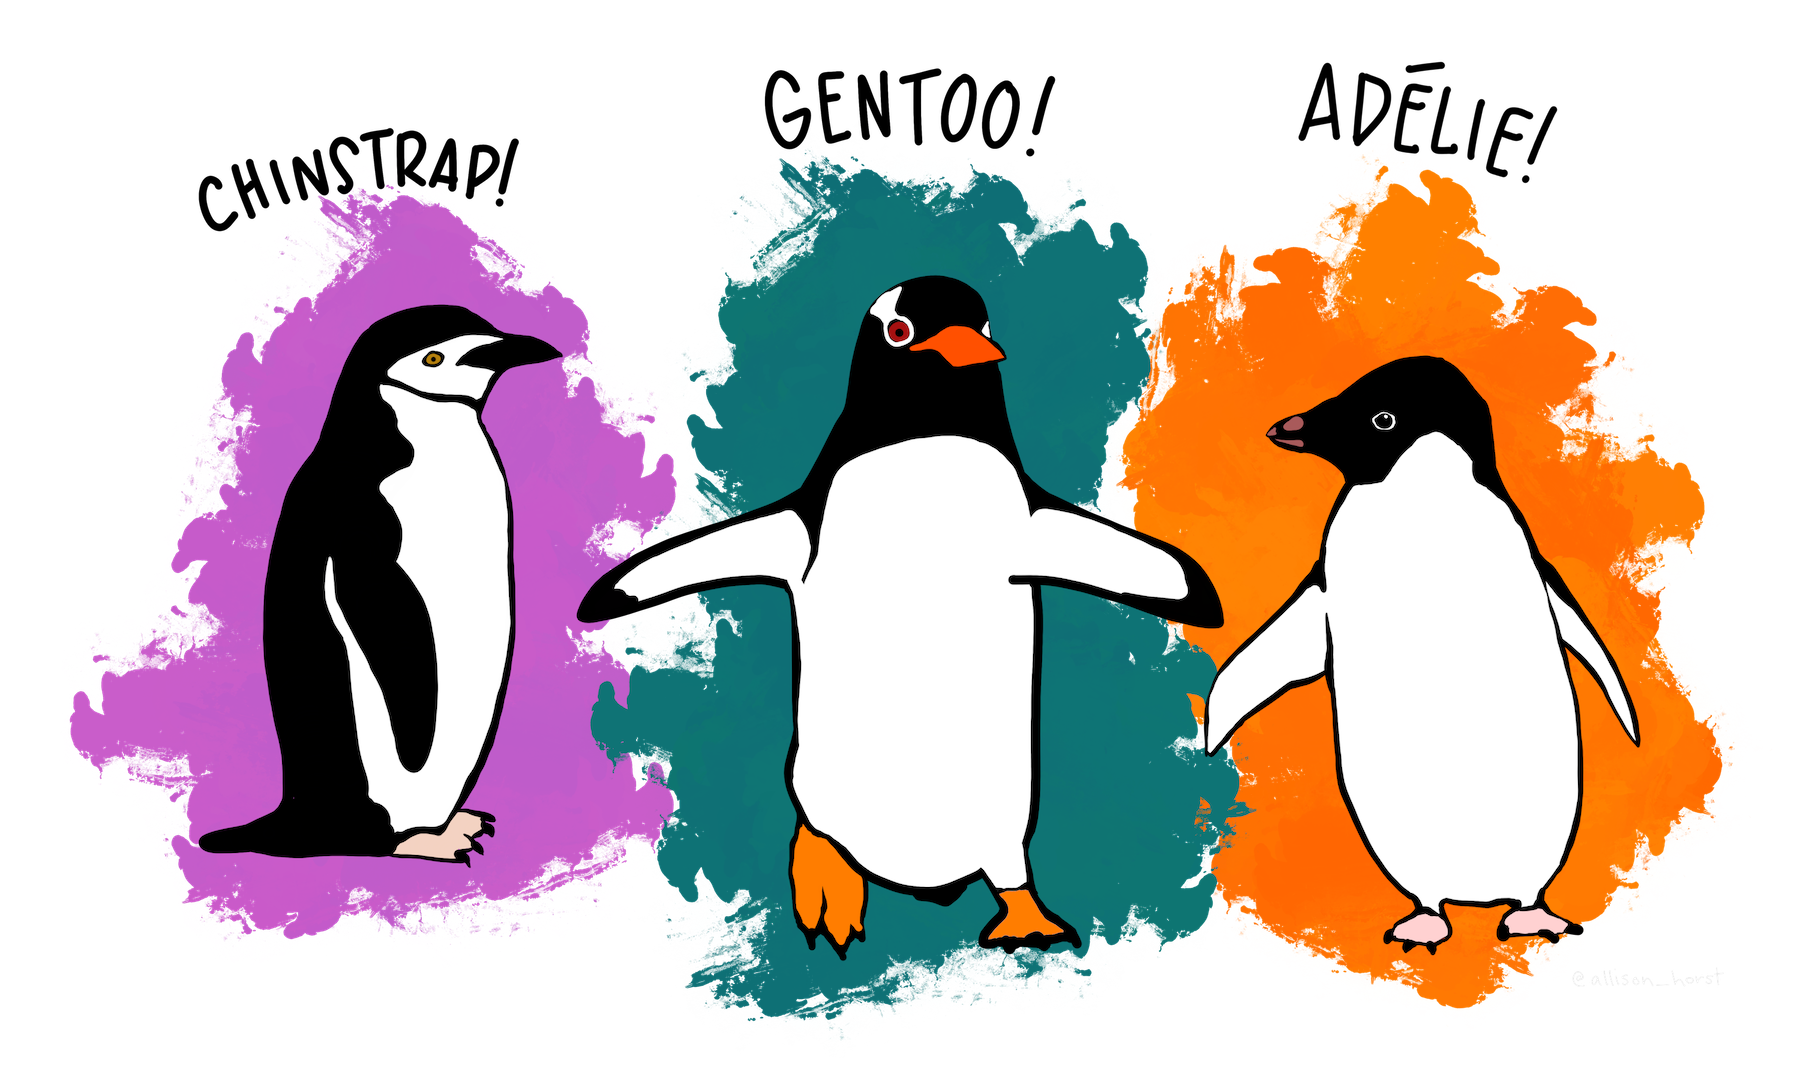
\includegraphics[width=0.5\textwidth,height=0.5\textheight]{./www/lter_penguins.png}

}

\caption{Artwork by allison\_horst}

\end{marginfigure}

\begin{Shaded}
\begin{Highlighting}[]
\FunctionTok{install.packages}\NormalTok{(}\StringTok{"palmerpenguins"}\NormalTok{)}
\FunctionTok{library}\NormalTok{(palmerpenguins)}
\end{Highlighting}
\end{Shaded}

Some of the graphs use datasets from the \texttt{fivethirtyeight}
package.

\begin{Shaded}
\begin{Highlighting}[]
\FunctionTok{install.packages}\NormalTok{(}\StringTok{"fivethirtyeight"}\NormalTok{)}
\FunctionTok{library}\NormalTok{(fivethirtyeight)}
\end{Highlighting}
\end{Shaded}

\begin{marginfigure}

{\centering 
\includegraphics[width=0.3\textwidth,height=0.3\textheight]{./www/538.png}

}

\end{marginfigure}

\begin{tcolorbox}[enhanced jigsaw, rightrule=.15mm, toprule=.15mm, opacityback=0, breakable, left=2mm, titlerule=0mm, bottomtitle=1mm, leftrule=.75mm, arc=.35mm, colback=white, toptitle=1mm, title={Expand to view the data in the \texttt{fivethirtyeight} package}, coltitle=black, colframe=quarto-callout-tip-color-frame, bottomrule=.15mm, opacitybacktitle=0.6, colbacktitle=quarto-callout-tip-color!10!white]

To view a table of available datasets in the \texttt{fivethirtyeight}
package, view the \texttt{Data\ Frame\ Name} and \texttt{Article\ Title}
columns in the \texttt{datasets\_master} table:

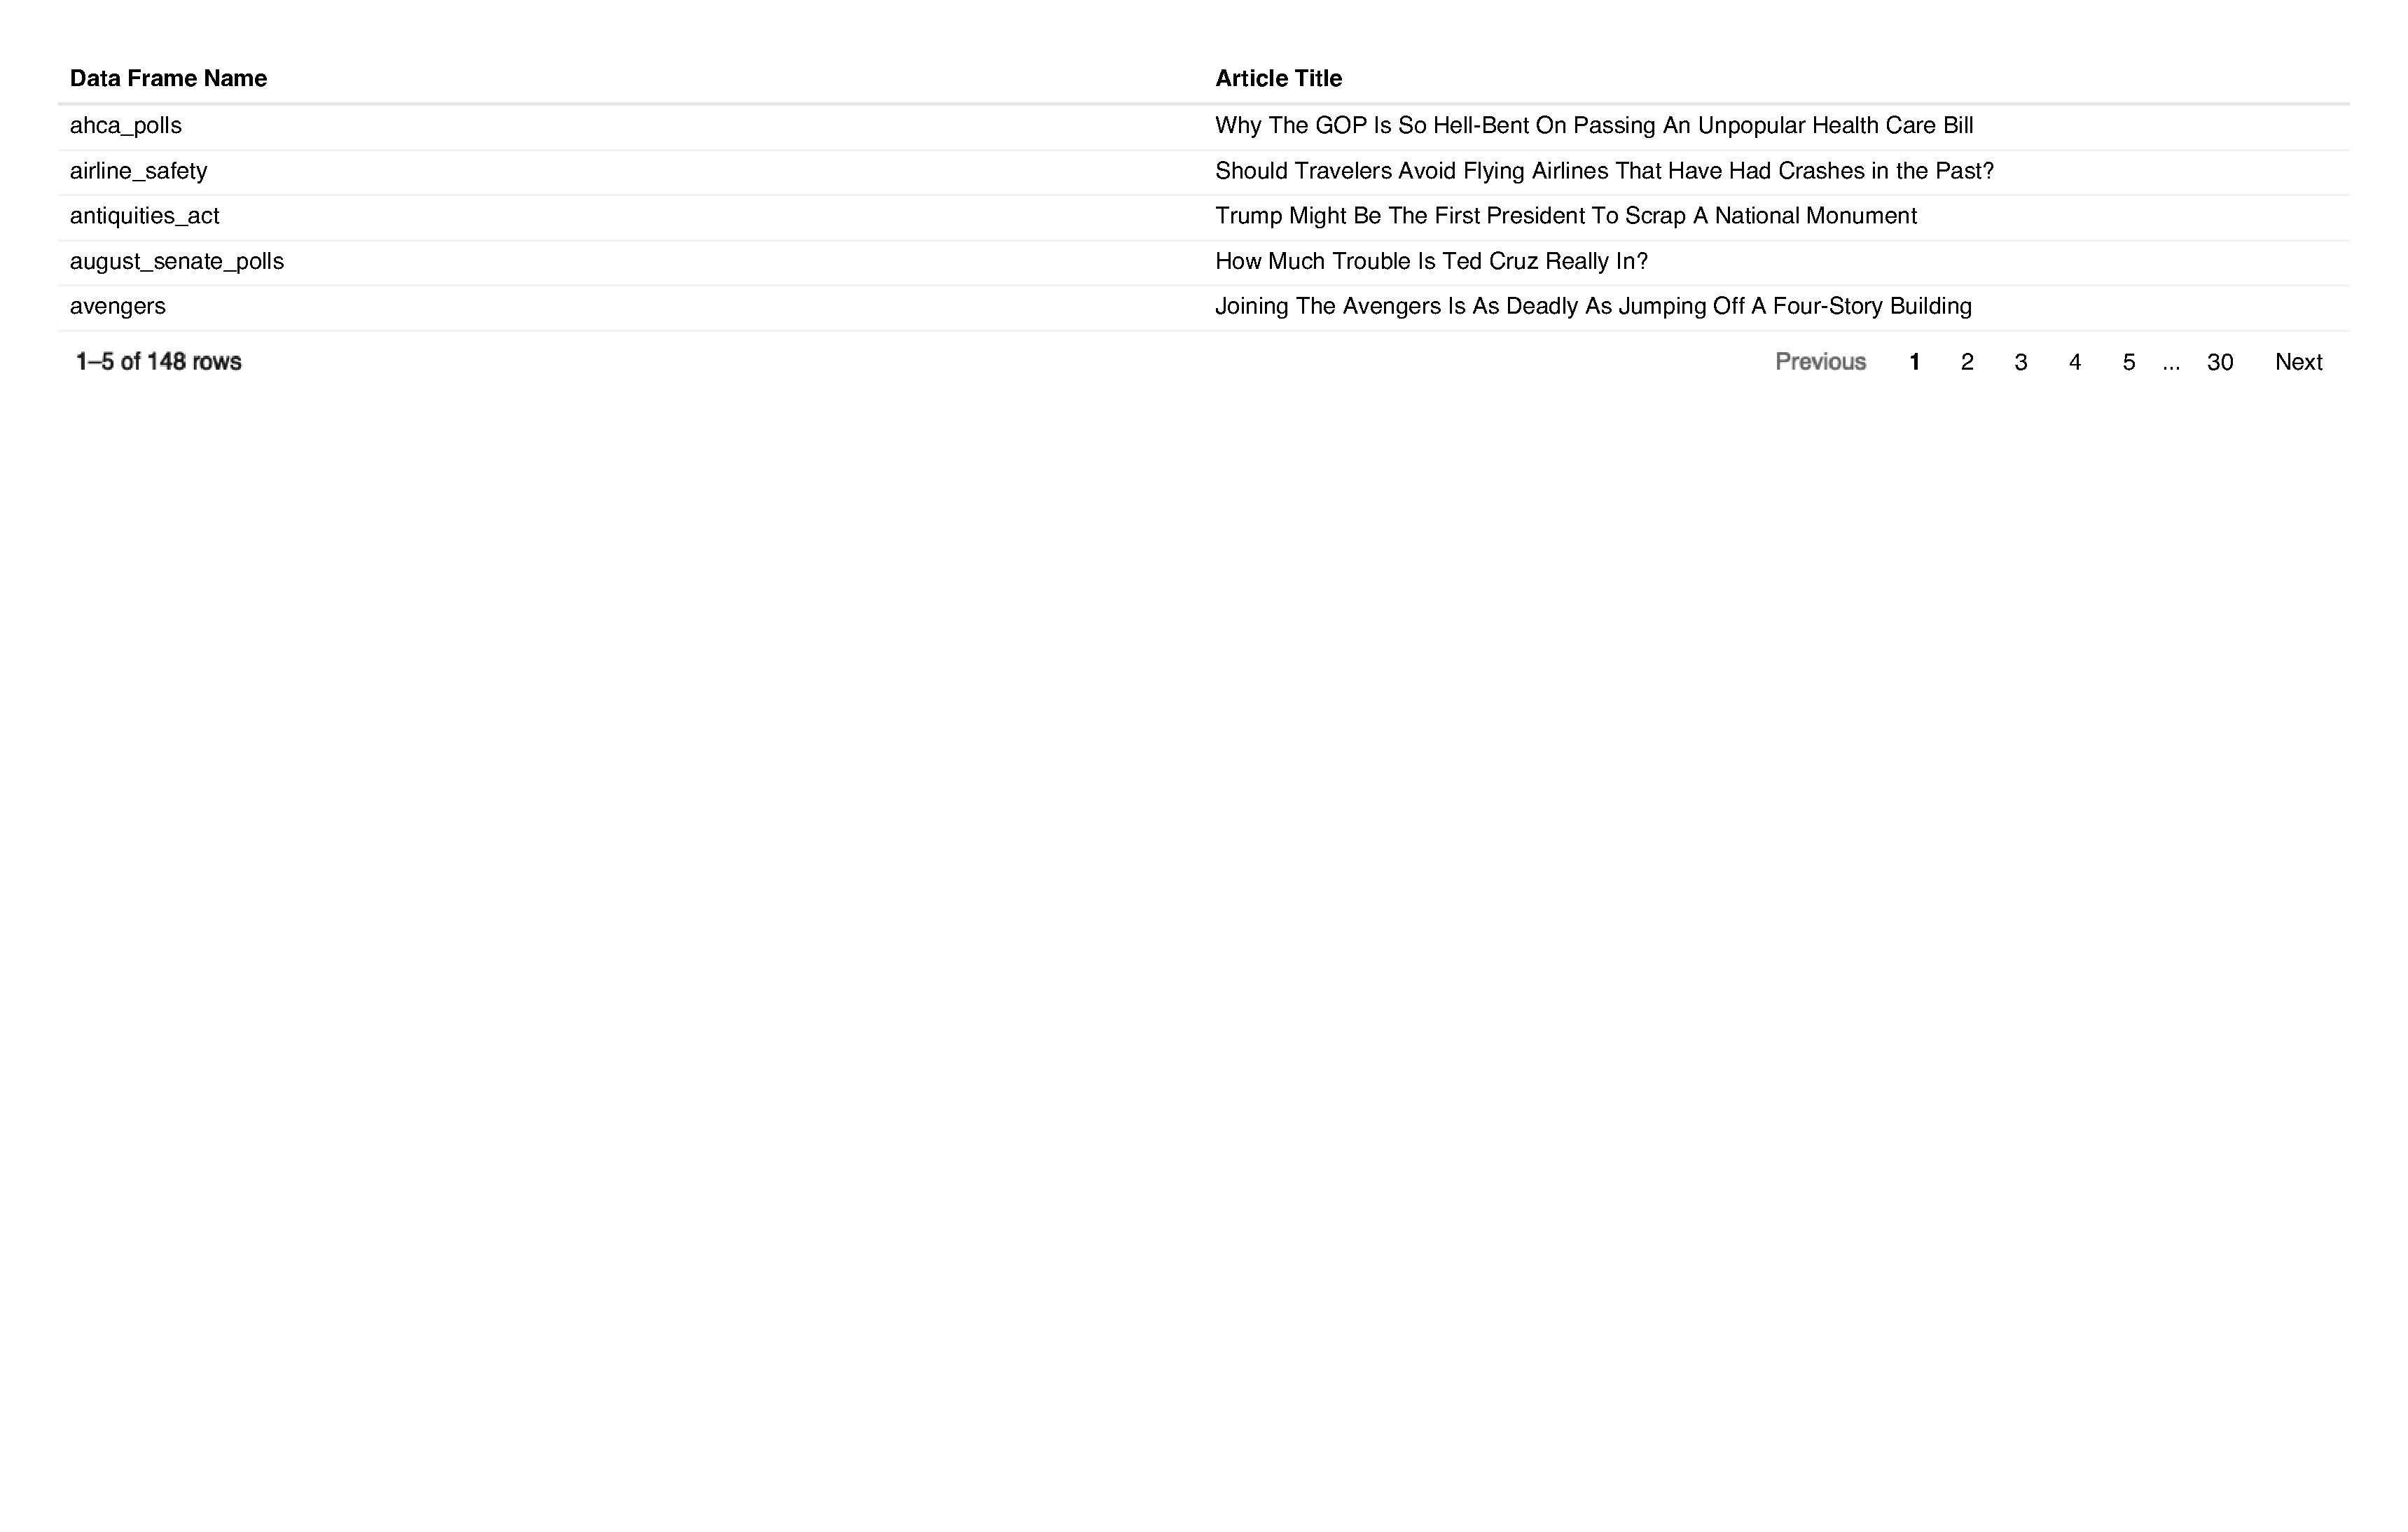
\includegraphics{./index_files/figure-pdf/538-pkg-1.pdf}

\end{tcolorbox}

A \emph{few} of the graphs are built using the
\texttt{ggplot2movies::movies} data.

\begin{marginfigure}

{\centering 
\includegraphics[width=0.3\textwidth,height=0.3\textheight]{./www/imdb.png}

}

\end{marginfigure}

\begin{Shaded}
\begin{Highlighting}[]
\FunctionTok{install.packages}\NormalTok{(}\StringTok{"ggplot2movies"}\NormalTok{)}
\FunctionTok{library}\NormalTok{(ggplot2movies)}
\end{Highlighting}
\end{Shaded}

\hypertarget{the-graphs}{%
\section*{The Graphs}\label{the-graphs}}
\addcontentsline{toc}{section}{The Graphs}

The gallery follows a
\href{https://www.w3.org/2001/tag/doc/leastPower.html}{Rule of Least
Power Principle}, in the sense that ``\emph{a language with a
straightforward syntax may be easier to analyze than an otherwise
equivalent one with more complex structure.}''

In other words, assuming the reader has some understanding of R and the
\texttt{tidyverse}, the code for each graph is meant to be read and
understood \emph{without} having to run it.

\hypertarget{graph-categories}{%
\subsection*{Graph Categories}\label{graph-categories}}
\addcontentsline{toc}{subsection}{Graph Categories}

Graphs have been categorized into the following types:

\begin{itemize}
\tightlist
\item
  Univariate graphs\\
\item
  Amounts
\item
  Proportions\\
\item
  Comparing Distributions\\
\item
  Relationships
\end{itemize}

Some graphs would justifiably belong in more than one category, and
wherever this is the case, I've tried to include links to other uses in
the notes.

\hypertarget{code-style-structure}{%
\section*{Code style \& structure}\label{code-style-structure}}
\addcontentsline{toc}{section}{Code style \& structure}

Each graph has, at minimum, the same two sections and four tabs:

\begin{enumerate}
\def\labelenumi{\arabic{enumi}.}
\tightlist
\item
  \textbf{Packages} and \textbf{Data}

  \begin{itemize}
  \tightlist
  \item
    Code for installing development version of packages (if necessary)
    for graphs \emph{and} data\\
  \item
    Any steps used to create (i.e., manipulate and prepare) the data for
    the graph\\
  \end{itemize}
\item
  \textbf{Code} and \textbf{Graph}

  \begin{itemize}
  \tightlist
  \item
    Code to build the labels and graph layers

    \begin{itemize}
    \tightlist
    \item
      \emph{Graph labels have the \texttt{labs\_} prefix}\\
    \item
      \emph{Graph layers have a \texttt{ggp2\_} prefix}
    \end{itemize}
  \end{itemize}
\end{enumerate}

\begin{tcolorbox}[enhanced jigsaw, rightrule=.15mm, toprule=.15mm, opacityback=0, breakable, left=2mm, titlerule=0mm, bottomtitle=1mm, leftrule=.75mm, arc=.35mm, colback=white, toptitle=1mm, title=\textcolor{quarto-callout-note-color}{\faInfo}\hspace{0.5em}{Expand to view the graph code structure}, coltitle=black, colframe=quarto-callout-note-color-frame, bottomrule=.15mm, opacitybacktitle=0.6, colbacktitle=quarto-callout-note-color!10!white]

\hypertarget{packages}{%
\subsubsection*{Packages}\label{packages}}
\addcontentsline{toc}{subsubsection}{Packages}

\textbf{PACKAGES:}

Install packages.

\begin{Shaded}
\begin{Highlighting}[]
\FunctionTok{library}\NormalTok{(ggplot2)}
\end{Highlighting}
\end{Shaded}

\hypertarget{data}{%
\subsubsection*{Data}\label{data}}
\addcontentsline{toc}{subsubsection}{Data}

\textbf{DATA:}

Description of data

\begin{Shaded}
\begin{Highlighting}[]
\NormalTok{df }\OtherTok{\textless{}{-}}\NormalTok{ tibble}\SpecialCharTok{::}\FunctionTok{tibble}\NormalTok{(}\AttributeTok{X =} \FunctionTok{sample}\NormalTok{(}\AttributeTok{x =} \DecValTok{1}\SpecialCharTok{:}\DecValTok{100}\NormalTok{, }\DecValTok{10}\NormalTok{, }\ConstantTok{FALSE}\NormalTok{),}
                     \AttributeTok{Y =} \FunctionTok{rlnorm}\NormalTok{(}\DecValTok{10}\NormalTok{, }\DecValTok{1}\NormalTok{, }\DecValTok{3}\NormalTok{))}
\end{Highlighting}
\end{Shaded}

\hypertarget{code}{%
\subsubsection*{Code}\label{code}}
\addcontentsline{toc}{subsubsection}{Code}

\textbf{CODE:}

Code for creating graph

\begin{Shaded}
\begin{Highlighting}[]
\CommentTok{\# labels}
\NormalTok{labs\_graph }\OtherTok{\textless{}{-}}\NormalTok{ ggplot2}\SpecialCharTok{::}\FunctionTok{labs}\NormalTok{(}\AttributeTok{title =} \StringTok{"Title"}\NormalTok{, }
                            \AttributeTok{subtitle =} \StringTok{"subtitle"}\NormalTok{, }
                            \AttributeTok{x =} \StringTok{"X"}\NormalTok{, }\AttributeTok{y =} \StringTok{"Y"}\NormalTok{)}
\CommentTok{\# layers}
\NormalTok{ggp2\_graph }\OtherTok{\textless{}{-}}\NormalTok{ ggplot2}\SpecialCharTok{::}\FunctionTok{ggplot}\NormalTok{(}\AttributeTok{data =}\NormalTok{ df, }
    \AttributeTok{mapping =} \FunctionTok{aes}\NormalTok{(}\AttributeTok{x =}\NormalTok{ X, }\AttributeTok{y =}\NormalTok{ Y)) }\SpecialCharTok{+} 
\NormalTok{    ggplot2}\SpecialCharTok{::}\FunctionTok{geom\_blank}\NormalTok{()}
\CommentTok{\# graph}
\NormalTok{ggp2\_graph }\SpecialCharTok{+} 
\NormalTok{    labs\_graph}
\end{Highlighting}
\end{Shaded}

\hypertarget{graph}{%
\subsubsection*{Graph}\label{graph}}
\addcontentsline{toc}{subsubsection}{Graph}

\textbf{GRAPH:}

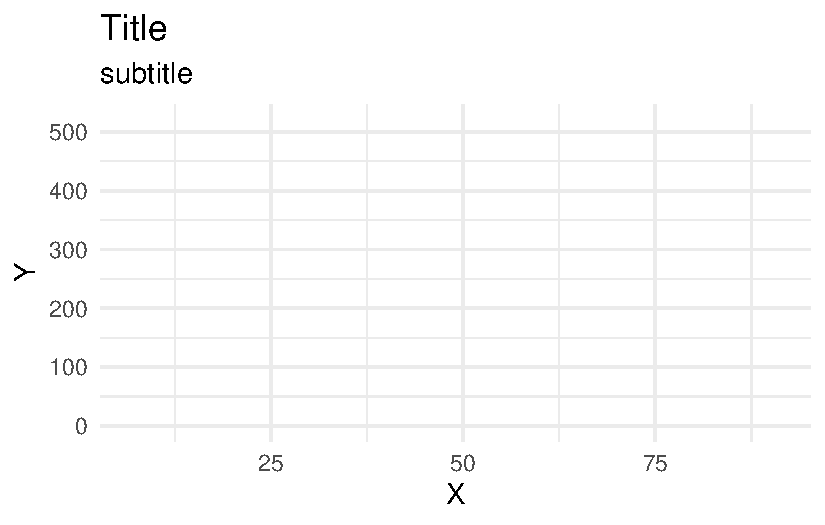
\includegraphics{./index_files/figure-pdf/create_graph_example-1.pdf}

\end{tcolorbox}

\textbf{Code Style:}

I've attempted to balance brevity and clarity, but with the assumption
that its best to err on the latter. I've also followed the general
principle that if a graph can be \emph{easily} built using one of
\texttt{ggplot2} 's \texttt{geom\_*} functions, that method is shown
first.

\hypertarget{extensions}{%
\section*{Extensions}\label{extensions}}
\addcontentsline{toc}{section}{Extensions}

Below are the graphs requiring additional packages/extensions:

\begin{itemize}
\item[$\boxtimes$]
  Waffle charts

  \begin{itemize}
  \item
    \href{https://liamgilbey.github.io/ggwaffle/}{\texttt{ggwaffle}
    package}

\begin{Shaded}
\begin{Highlighting}[]
\CommentTok{\# Waffle Charts}
\NormalTok{devtools}\SpecialCharTok{::}\FunctionTok{install\_github}\NormalTok{(}\StringTok{"liamgilbey/ggwaffle"}\NormalTok{)}
\FunctionTok{library}\NormalTok{(ggwaffle)}
\end{Highlighting}
\end{Shaded}
  \end{itemize}
\item[$\boxtimes$]
  Pie Charts

  \begin{itemize}
  \item
    \href{https://rpkgs.datanovia.com/ggpubr/}{\texttt{ggpubr} package}

\begin{Shaded}
\begin{Highlighting}[]
\CommentTok{\# Pie Charts }
\NormalTok{devtools}\SpecialCharTok{::}\FunctionTok{install\_github}\NormalTok{(}\StringTok{"kassambara/ggpubr"}\NormalTok{)}
\FunctionTok{library}\NormalTok{(ggpubr)}
\end{Highlighting}
\end{Shaded}
  \end{itemize}
\item[$\boxtimes$]
  Mosaic Plots

  \begin{itemize}
  \item
    \href{https://haleyjeppson.github.io/ggmosaic/}{\texttt{ggmosaic}
    package}

\begin{Shaded}
\begin{Highlighting}[]
\CommentTok{\# Mosaic Charts }
\NormalTok{devtools}\SpecialCharTok{::}\FunctionTok{install\_github}\NormalTok{(}\StringTok{"haleyjeppson/ggmosaic"}\NormalTok{)}
\FunctionTok{library}\NormalTok{(ggmosaic)}
\end{Highlighting}
\end{Shaded}
  \end{itemize}
\item[$\boxtimes$]
  Treemaps

  \begin{itemize}
  \item
    \href{https://wilkox.org/treemapify/}{\texttt{treemapify} package}

\begin{Shaded}
\begin{Highlighting}[]
\CommentTok{\# Treemaps}
\NormalTok{devtools}\SpecialCharTok{::}\FunctionTok{install\_github}\NormalTok{(}\StringTok{"wilkox/treemapify"}\NormalTok{)}
\FunctionTok{library}\NormalTok{(treemapify)}
\end{Highlighting}
\end{Shaded}
  \end{itemize}
\item[$\boxtimes$]
  Bee-swarm Plots

  \begin{itemize}
  \item
    \href{https://github.com/eclarke/ggbeeswarm}{\texttt{ggbeeswarm}
    package}

\begin{Shaded}
\begin{Highlighting}[]
\CommentTok{\# Bee{-}swarm Plots}
\NormalTok{devtools}\SpecialCharTok{::}\FunctionTok{install\_github}\NormalTok{(}\StringTok{"eclarke/ggbeeswarm"}\NormalTok{)}
\FunctionTok{library}\NormalTok{(ggbeeswarm)}
\end{Highlighting}
\end{Shaded}
  \end{itemize}
\item[$\boxtimes$]
  Ridgeline Plots

  \begin{itemize}
  \item
    \href{https://wilkelab.org/ggridges/}{\texttt{ggridges} package}

\begin{Shaded}
\begin{Highlighting}[]
\CommentTok{\# Ridgeline plots }
\NormalTok{devtools}\SpecialCharTok{::}\FunctionTok{install\_github}\NormalTok{(}\StringTok{"wilkelab/ggridges"}\NormalTok{)}
\FunctionTok{library}\NormalTok{(ggridges)}
\end{Highlighting}
\end{Shaded}
  \end{itemize}
\item[$\boxtimes$]
  Rain-cloud plots

  \begin{itemize}
  \item
    \href{https://github.com/jorvlan/raincloudplots}{\texttt{raincloudplots}}
    and
    \href{https://mjskay.github.io/ggdist/reference/index.html}{\texttt{ggdist}}
    packages

\begin{Shaded}
\begin{Highlighting}[]
\CommentTok{\# Rain{-}cloud plots }
\NormalTok{remotes}\SpecialCharTok{::}\FunctionTok{install\_github}\NormalTok{(}\StringTok{\textquotesingle{}jorvlan/raincloudplots\textquotesingle{}}\NormalTok{)}
\NormalTok{remotes}\SpecialCharTok{::}\FunctionTok{install\_github}\NormalTok{(}\StringTok{\textquotesingle{}mjskay/ggdist\textquotesingle{}}\NormalTok{)}
\FunctionTok{library}\NormalTok{(raincloudplots)}
\FunctionTok{library}\NormalTok{(ggdist)}
\end{Highlighting}
\end{Shaded}
  \end{itemize}
\item[$\boxtimes$]
  Alluvial charts

  \begin{itemize}
  \item
    \href{https://corybrunson.github.io/ggalluvial/}{ggalluvial package}

\begin{Shaded}
\begin{Highlighting}[]
\CommentTok{\# Alluvial charts}
\NormalTok{devtools}\SpecialCharTok{::}\FunctionTok{install\_github}\NormalTok{(}\StringTok{"corybrunson/ggalluvial"}\NormalTok{)}
\FunctionTok{library}\NormalTok{(ggalluvial)}
\end{Highlighting}
\end{Shaded}
  \end{itemize}
\item[$\boxtimes$]
  Bump charts

  \begin{itemize}
  \item
    \href{https://github.com/davidsjoberg/ggbump}{ggbump package}

\begin{Shaded}
\begin{Highlighting}[]
\CommentTok{\# Bump charts}
\NormalTok{devtools}\SpecialCharTok{::}\FunctionTok{install\_github}\NormalTok{(}\StringTok{"davidsjoberg/ggbump"}\NormalTok{)}
\FunctionTok{library}\NormalTok{(ggbump)}
\end{Highlighting}
\end{Shaded}
  \end{itemize}
\item[$\boxtimes$]
  Parallel Sets

  \begin{itemize}
  \item
    \href{https://ggforce.data-imaginist.com/index.html}{ggforce
    package}

\begin{Shaded}
\begin{Highlighting}[]
\CommentTok{\# Bump charts}
\NormalTok{devtools}\SpecialCharTok{::}\FunctionTok{install\_github}\NormalTok{(}\StringTok{"thomasp85/ggforce"}\NormalTok{)}
\FunctionTok{library}\NormalTok{(ggforce)}
\end{Highlighting}
\end{Shaded}
  \end{itemize}
\item[$\boxtimes$]
  Stream Plots

  \begin{itemize}
  \item
    \href{https://github.com/davidsjoberg/ggstream}{ggstream package}

\begin{Shaded}
\begin{Highlighting}[]
\CommentTok{\# Stream plots}
\NormalTok{devtools}\SpecialCharTok{::}\FunctionTok{install\_github}\NormalTok{(}\StringTok{"davidsjoberg/ggstream"}\NormalTok{)}
\FunctionTok{library}\NormalTok{(ggstream)}
\end{Highlighting}
\end{Shaded}
  \end{itemize}
\end{itemize}

\hypertarget{theme}{%
\section*{Theme}\label{theme}}
\addcontentsline{toc}{section}{Theme}

The theme used in the graphs is custom and uses combined elements from
\texttt{ggplot2::theme\_minimal()} and \texttt{ggplot2::theme\_void()}.
View it
\href{https://github.com/mjfrigaard/ggp2-gallery/blob/main/R/theme_ggp2g.R}{here}.

\part{Univariate}

\hypertarget{bar-graphs}{%
\chapter*{Bar graphs}\label{bar-graphs}}
\addcontentsline{toc}{chapter}{Bar graphs}

\begin{tcolorbox}[enhanced jigsaw, rightrule=.15mm, toprule=.15mm, opacityback=0, breakable, left=2mm, titlerule=0mm, bottomtitle=1mm, leftrule=.75mm, arc=.35mm, colback=white, toptitle=1mm, title={Graph info}, coltitle=black, colframe=quarto-callout-note-color-frame, bottomrule=.15mm, opacitybacktitle=0.6, colbacktitle=quarto-callout-note-color!10!white]

\textbf{Should I use this graph?}

\begin{figure}

\hfill{} 
\includegraphics[width=0.6\textwidth,height=0.6\textheight]{uni/bar_graphs_files/figure-pdf/full_code_display-1.pdf}

\end{figure}

\textbf{This graph requires:}

✅ a categorical variable

\end{tcolorbox}

\hypertarget{description}{%
\section*{Description}\label{description}}
\addcontentsline{toc}{section}{Description}

A bar graph (or bar chart) is typically used to display counts for the
discrete levels of a categorical variable, like political affiliation,
hair color, or race/ethnicity (or species of penguin!).

Bar graphs can be arranged vertically or horizontally, but the length of
the bar represents the `count' for each category value.

In \texttt{ggplot2}, bar graphs can be built using \texttt{geom\_bar()}
(see also:
\href{https://mjfrigaard.github.io/ggp2-gallery/geoms/geom_col.html}{\texttt{geom\_col()}}).

\hypertarget{getting-set-up}{%
\section*{Getting set up}\label{getting-set-up}}
\addcontentsline{toc}{section}{Getting set up}

\hypertarget{packages-1}{%
\subsubsection*{Packages}\label{packages-1}}
\addcontentsline{toc}{subsubsection}{Packages}

\textbf{PACKAGES:}

Install packages.

\begin{Shaded}
\begin{Highlighting}[]
\FunctionTok{install.packages}\NormalTok{(}\StringTok{"palmerpenguins"}\NormalTok{)}
\FunctionTok{library}\NormalTok{(palmerpenguins) }
\FunctionTok{library}\NormalTok{(ggplot2)}
\end{Highlighting}
\end{Shaded}

\hypertarget{data-1}{%
\subsubsection*{Data}\label{data-1}}
\addcontentsline{toc}{subsubsection}{Data}

\textbf{DATA:}

\begin{marginfigure}

\hfill{} \includegraphics[width=1\textwidth,height=1\textheight]{uni/../www/lter_penguins.png}

\caption{Artwork by Allison Horst}

\end{marginfigure}

Filter the missing values from \texttt{species} in the
\texttt{palmerpenguins::penguins} data and store it in
\texttt{penguins\_bar}.

\begin{Shaded}
\begin{Highlighting}[]
\NormalTok{penguins\_bar }\OtherTok{\textless{}{-}}\NormalTok{ palmerpenguins}\SpecialCharTok{::}\NormalTok{penguins }\SpecialCharTok{|\textgreater{}} 
\NormalTok{    dplyr}\SpecialCharTok{::}\FunctionTok{filter}\NormalTok{(}\SpecialCharTok{!}\FunctionTok{is.na}\NormalTok{(species))}
\FunctionTok{glimpse}\NormalTok{(penguins\_bar)}
\end{Highlighting}
\end{Shaded}

\begin{verbatim}
Rows: 344
Columns: 8
$ species           <fct> Adelie, Adelie, Adelie, Adelie, Adelie, Adelie, Adel~
$ island            <fct> Torgersen, Torgersen, Torgersen, Torgersen, Torgerse~
$ bill_length_mm    <dbl> 39.1, 39.5, 40.3, NA, 36.7, 39.3, 38.9, 39.2, 34.1, ~
$ bill_depth_mm     <dbl> 18.7, 17.4, 18.0, NA, 19.3, 20.6, 17.8, 19.6, 18.1, ~
$ flipper_length_mm <int> 181, 186, 195, NA, 193, 190, 181, 195, 193, 190, 186~
$ body_mass_g       <int> 3750, 3800, 3250, NA, 3450, 3650, 3625, 4675, 3475, ~
$ sex               <fct> male, female, female, NA, female, male, female, male~
$ year              <int> 2007, 2007, 2007, 2007, 2007, 2007, 2007, 2007, 2007~
\end{verbatim}

\hypertarget{the-grammar}{%
\section*{The grammar}\label{the-grammar}}
\addcontentsline{toc}{section}{The grammar}

\hypertarget{code-1}{%
\subsubsection*{Code}\label{code-1}}
\addcontentsline{toc}{subsubsection}{Code}

\textbf{CODE:}

Create labels with \texttt{labs()}

Initialize the graph with \texttt{ggplot()} and provide \texttt{data}

Map \texttt{species} to the \texttt{x} axis

Map \texttt{species} to the \texttt{fill} aesthetic inside the
\texttt{aes()} of \texttt{geom\_bar()}

Remove the legend with \texttt{show.legend\ =\ FALSE}

\begin{Shaded}
\begin{Highlighting}[]
\NormalTok{labs\_bar }\OtherTok{\textless{}{-}} \FunctionTok{labs}\NormalTok{(}
  \AttributeTok{title =} \StringTok{"Adult foraging penguins"}\NormalTok{,}
  \AttributeTok{subtitle =} \StringTok{"Distribution of flipper length"}\NormalTok{,}
  \AttributeTok{x =} \StringTok{"Species"}\NormalTok{, }\AttributeTok{y =} \StringTok{"Count"}\NormalTok{, }
  \AttributeTok{fill =} \StringTok{"Species"}\NormalTok{)}
\NormalTok{ggp2\_bar }\OtherTok{\textless{}{-}} \FunctionTok{ggplot}\NormalTok{(}\AttributeTok{data =}\NormalTok{ penguins\_bar,}
       \FunctionTok{aes}\NormalTok{(}\AttributeTok{x =}\NormalTok{ species)) }\SpecialCharTok{+}
    \FunctionTok{geom\_bar}\NormalTok{(}\FunctionTok{aes}\NormalTok{(}\AttributeTok{fill =}\NormalTok{ species), }
        \AttributeTok{show.legend =} \ConstantTok{FALSE}\NormalTok{)}
\NormalTok{ggp2\_bar }\SpecialCharTok{+}
\NormalTok{  labs\_bar}
\end{Highlighting}
\end{Shaded}

\hypertarget{graph-1}{%
\subsubsection*{Graph}\label{graph-1}}
\addcontentsline{toc}{subsubsection}{Graph}

\textbf{GRAPH:}


\includegraphics[width=1\textwidth,height=1\textheight]{uni/bar_graphs_files/figure-pdf/create_graph_bar-1.pdf}

\hypertarget{more-info}{%
\section*{More info}\label{more-info}}
\addcontentsline{toc}{section}{More info}

\begin{itemize}
\tightlist
\item
  The connection between statistical transformations and geoms is an
  important principle for building graphs (and mastering the grammar)
  with \texttt{ggplot2}

  \begin{itemize}
  \tightlist
  \item
    Below we cover why \texttt{geom\_bar(stat\ =\ "count")} produces the
    same result as \texttt{stat\_count(geom\ =\ "bar")}
  \end{itemize}
\end{itemize}

\marginnote{\begin{footnotesize}

``\emph{every geom has a default stat, and every stat a default geom.}''
- \href{https://ggplot2-book.org/layers.html\#layers}{\texttt{ggplot2}
book}

\end{footnotesize}}

\begin{itemize}
\tightlist
\item
  Bar graphs can also be created with \texttt{geom\_col()}
\end{itemize}

\hypertarget{stats-and-geoms}{%
\subsubsection*{stats and geoms}\label{stats-and-geoms}}
\addcontentsline{toc}{subsubsection}{stats and geoms}

\textbf{stat\_count():}

The default \texttt{stat} argument in \texttt{geom\_bar()} is set to
\texttt{"count"}, which `\emph{counts the number of cases at each
\texttt{x} position}', so it's ideal for categorical variables (or
factors).

The \texttt{stat\_count()} function can also be used to create bar
graphs using the \texttt{geom} argument.

The link between
\texttt{geom\_}\textbf{geom\_name}\texttt{(stat\ =\ "}\textbf{stat\_name}\texttt{")}
and
\texttt{stat\_}\textbf{stat\_name}\texttt{(geom\ =\ "}\textbf{geom\_name}\texttt{")}
is shown below:

\begin{Shaded}
\begin{Highlighting}[]
\NormalTok{ggp2\_geom\_bar }\OtherTok{\textless{}{-}} \FunctionTok{ggplot}\NormalTok{(}\AttributeTok{data =}\NormalTok{ penguins\_bar,}
       \FunctionTok{aes}\NormalTok{(}\AttributeTok{x =}\NormalTok{ species)) }\SpecialCharTok{+}
    \FunctionTok{geom\_bar}\NormalTok{(}\FunctionTok{aes}\NormalTok{(}\AttributeTok{fill =}\NormalTok{ species), }
        \AttributeTok{stat =} \StringTok{"count"}\NormalTok{) }\SpecialCharTok{+} 
    \FunctionTok{labs}\NormalTok{(}\AttributeTok{title =} \StringTok{"geom\_bar(stat = \textquotesingle{}count\textquotesingle{})"}\NormalTok{)}
\NormalTok{ggp2\_geom\_bar}
\end{Highlighting}
\end{Shaded}

\begin{figure}[H]

{\centering 
\includegraphics[width=1\textwidth,height=1\textheight]{uni/bar_graphs_files/figure-pdf/stat_vs_geom_bar-1.pdf}

}

\end{figure}

\begin{Shaded}
\begin{Highlighting}[]
\NormalTok{ggp2\_stat\_count }\OtherTok{\textless{}{-}} \FunctionTok{ggplot}\NormalTok{(}\AttributeTok{data =}\NormalTok{ penguins\_bar,}
       \FunctionTok{aes}\NormalTok{(}\AttributeTok{x =}\NormalTok{ species)) }\SpecialCharTok{+}
    \FunctionTok{stat\_count}\NormalTok{(}\FunctionTok{aes}\NormalTok{(}\AttributeTok{fill =}\NormalTok{ species), }
        \AttributeTok{geom =} \StringTok{"bar"}\NormalTok{) }\SpecialCharTok{+} 
    \FunctionTok{labs}\NormalTok{(}\AttributeTok{title =} \StringTok{"stat\_count(geom = \textquotesingle{}bar\textquotesingle{})"}\NormalTok{)}
\NormalTok{ggp2\_stat\_count}
\end{Highlighting}
\end{Shaded}

\begin{figure}[H]

{\centering 
\includegraphics[width=1\textwidth,height=1\textheight]{uni/bar_graphs_files/figure-pdf/stat_vs_geom_bar-2.pdf}

}

\end{figure}

\hypertarget{geom_col}{%
\subsubsection*{\texorpdfstring{\texttt{geom\_col()}}{geom\_col()}}\label{geom_col}}
\addcontentsline{toc}{subsubsection}{\texttt{geom\_col()}}

\textbf{geom\_col:}

To create a bar graph with \texttt{geom\_col()}, the \texttt{count}
variable needs to be computed before being mapped into the graph
\texttt{y} aesthetic.

\begin{Shaded}
\begin{Highlighting}[]
\NormalTok{penguins\_bar }\SpecialCharTok{|\textgreater{}} 
    \CommentTok{\# create column of counts }
\NormalTok{    dplyr}\SpecialCharTok{::}\FunctionTok{count}\NormalTok{(species, }\AttributeTok{name =} \StringTok{"count"}\NormalTok{) }\SpecialCharTok{|\textgreater{}} 
    \CommentTok{\# map into x and y}
    \FunctionTok{ggplot}\NormalTok{(}\AttributeTok{mapping =} \FunctionTok{aes}\NormalTok{(}\AttributeTok{x =}\NormalTok{ species, }\AttributeTok{y =}\NormalTok{ count)) }\SpecialCharTok{+}
    \FunctionTok{geom\_col}\NormalTok{(}\FunctionTok{aes}\NormalTok{(}\AttributeTok{fill =}\NormalTok{ species), }
        \AttributeTok{show.legend =} \ConstantTok{FALSE}\NormalTok{) }\SpecialCharTok{+} 
\NormalTok{    labs\_bar }\SpecialCharTok{+}
    \FunctionTok{labs}\NormalTok{(}\AttributeTok{caption =} \StringTok{"*created with geom\_col()"}\NormalTok{)}
\end{Highlighting}
\end{Shaded}

\begin{figure}[H]

{\centering 
\includegraphics[width=1\textwidth,height=1\textheight]{uni/bar_graphs_files/figure-pdf/bar_with_geom_col-1.pdf}

}

\end{figure}

\begin{Shaded}
\begin{Highlighting}[]
\CommentTok{\# compare to geom\_bar()}
\NormalTok{ggp2\_bar }\SpecialCharTok{+}
\NormalTok{  labs\_bar}
\end{Highlighting}
\end{Shaded}

\begin{figure}[H]

{\centering 
\includegraphics[width=1\textwidth,height=1\textheight]{uni/bar_graphs_files/figure-pdf/bar_with_geom_col-2.pdf}

}

\end{figure}

\hypertarget{histograms}{%
\chapter*{Histograms}\label{histograms}}
\addcontentsline{toc}{chapter}{Histograms}

\begin{tcolorbox}[enhanced jigsaw, rightrule=.15mm, toprule=.15mm, opacityback=0, breakable, left=2mm, titlerule=0mm, bottomtitle=1mm, leftrule=.75mm, arc=.35mm, colback=white, toptitle=1mm, title={Graph info}, coltitle=black, colframe=quarto-callout-note-color-frame, bottomrule=.15mm, opacitybacktitle=0.6, colbacktitle=quarto-callout-note-color!10!white]

\textbf{Should I use this graph?}

\begin{figure}

\hfill{} 
\includegraphics[width=0.6\textwidth,height=0.6\textheight]{uni/histograms_files/figure-pdf/full_code_display-1.pdf}

\end{figure}

\textbf{This graph requires:}

✅ a numeric (continuous) variable

\end{tcolorbox}

\hypertarget{description-1}{%
\section*{Description}\label{description-1}}
\addcontentsline{toc}{section}{Description}

Histograms are a special kind of bar graph. The \texttt{x} axis is
divided into `bins' that cover the range of a variable's values, and the
height of the bars is the frequency (or count) of the value occurrence
(displayed on the \texttt{y} axis).

Unlike a typical bar graph, histograms can be used to visually asses the
`\href{https://en.wikipedia.org/wiki/Normal_distribution}{normality}'
(i.e.~\emph{are the bars symmetrical, with a single peak in the middle
of the \texttt{x} axis?} Or \emph{do the bars form multiple peaks?}) or
`\href{https://en.wikipedia.org/wiki/Skewness}{skewness}' (i.e.,
\emph{is there a long `tail' of bars with decreasing length on either
end of the \texttt{x} axis?}) of a variable's distribution.

\hypertarget{getting-set-up-1}{%
\section*{Getting set up}\label{getting-set-up-1}}
\addcontentsline{toc}{section}{Getting set up}

\hypertarget{packages-2}{%
\subsubsection*{Packages}\label{packages-2}}
\addcontentsline{toc}{subsubsection}{Packages}

\textbf{PACKAGES:}

Install packages.

\begin{Shaded}
\begin{Highlighting}[]
\FunctionTok{install.packages}\NormalTok{(}\StringTok{"palmerpenguins"}\NormalTok{)}
\FunctionTok{library}\NormalTok{(palmerpenguins) }
\FunctionTok{library}\NormalTok{(ggplot2)}
\end{Highlighting}
\end{Shaded}

\hypertarget{data-2}{%
\subsubsection*{Data}\label{data-2}}
\addcontentsline{toc}{subsubsection}{Data}

\textbf{DATA:}

\begin{marginfigure}

\hfill{} \includegraphics[width=1\textwidth,height=1\textheight]{uni/../www/lter_penguins.png}

\caption{Artwork by Allison Horst}

\end{marginfigure}

The \texttt{penguins} data.

\begin{Shaded}
\begin{Highlighting}[]
\NormalTok{penguins }\OtherTok{\textless{}{-}}\NormalTok{ palmerpenguins}\SpecialCharTok{::}\NormalTok{penguins}
\FunctionTok{glimpse}\NormalTok{(penguins)}
\end{Highlighting}
\end{Shaded}

\begin{verbatim}
Rows: 344
Columns: 8
$ species           <fct> Adelie, Adelie, Adelie, Adelie, Adelie, Adelie, Adel~
$ island            <fct> Torgersen, Torgersen, Torgersen, Torgersen, Torgerse~
$ bill_length_mm    <dbl> 39.1, 39.5, 40.3, NA, 36.7, 39.3, 38.9, 39.2, 34.1, ~
$ bill_depth_mm     <dbl> 18.7, 17.4, 18.0, NA, 19.3, 20.6, 17.8, 19.6, 18.1, ~
$ flipper_length_mm <int> 181, 186, 195, NA, 193, 190, 181, 195, 193, 190, 186~
$ body_mass_g       <int> 3750, 3800, 3250, NA, 3450, 3650, 3625, 4675, 3475, ~
$ sex               <fct> male, female, female, NA, female, male, female, male~
$ year              <int> 2007, 2007, 2007, 2007, 2007, 2007, 2007, 2007, 2007~
\end{verbatim}

\hypertarget{the-grammar-1}{%
\section*{The grammar}\label{the-grammar-1}}
\addcontentsline{toc}{section}{The grammar}

\hypertarget{code-2}{%
\subsubsection*{Code}\label{code-2}}
\addcontentsline{toc}{subsubsection}{Code}

\textbf{CODE:}

Create labels with \texttt{labs()}

Initialize the graph with \texttt{ggplot()} and provide \texttt{data}

Assign \texttt{flipper\_length\_mm} to the \texttt{x}

Add the \texttt{geom\_histogram()}

Adjust the \texttt{bins} accordingly

\begin{Shaded}
\begin{Highlighting}[]
\NormalTok{labs\_histogram }\OtherTok{\textless{}{-}} \FunctionTok{labs}\NormalTok{(}
  \AttributeTok{title =} \StringTok{"Adult foraging penguins"}\NormalTok{,}
  \AttributeTok{subtitle =} \StringTok{"Distribution of flipper length"}\NormalTok{,}
  \AttributeTok{x =} \StringTok{"Flipper length (millimeters)"}\NormalTok{)}

\NormalTok{ggp2\_hist }\OtherTok{\textless{}{-}} \FunctionTok{ggplot}\NormalTok{(}\AttributeTok{data =}\NormalTok{ penguins,}
     \FunctionTok{aes}\NormalTok{(}\AttributeTok{x =}\NormalTok{ flipper\_length\_mm)) }\SpecialCharTok{+} 
     \FunctionTok{geom\_histogram}\NormalTok{() }

\NormalTok{ggp2\_hist }\SpecialCharTok{+} 
\NormalTok{  labs\_histogram}
\end{Highlighting}
\end{Shaded}

\hypertarget{graph-2}{%
\subsubsection*{Graph}\label{graph-2}}
\addcontentsline{toc}{subsubsection}{Graph}

\textbf{GRAPH:}


\includegraphics{uni/histograms_files/figure-pdf/create_graph_histogram-1.pdf}

The standard number of bins is \texttt{30}, but
\href{https://ggplot2.tidyverse.org/reference/geom_histogram.html}{`you
should always override this value, exploring multiple widths to find the
best to illustrate the stories in your data.'}

\part{Amounts}

\hypertarget{chapter-1}{%
\chapter{Chapter 1}\label{chapter-1}}

Placeholder for chapter 1.

See Knuth (1984) for additional discussion of literate programming.

\begin{Shaded}
\begin{Highlighting}[]
\DecValTok{1} \SpecialCharTok{+} \DecValTok{1}
\end{Highlighting}
\end{Shaded}

\begin{verbatim}
[1] 2
\end{verbatim}

\part{Proportions}

\hypertarget{chapter-2}{%
\chapter{Chapter 2}\label{chapter-2}}

Placeholder for chapter 2.

See Knuth (1984) for additional discussion of literate programming.

\begin{Shaded}
\begin{Highlighting}[]
\DecValTok{2} \SpecialCharTok{+} \DecValTok{2}
\end{Highlighting}
\end{Shaded}

\begin{verbatim}
[1] 4
\end{verbatim}

\part{Distributions}

\hypertarget{chapter-3}{%
\chapter{Chapter 3}\label{chapter-3}}

Placeholder for chapter 3.

See Knuth (1984) for additional discussion of literate programming.

\begin{Shaded}
\begin{Highlighting}[]
\DecValTok{3} \SpecialCharTok{+} \DecValTok{3}
\end{Highlighting}
\end{Shaded}

\begin{verbatim}
[1] 6
\end{verbatim}

\part{Relationships}

\hypertarget{chapter-4}{%
\chapter{Chapter 4}\label{chapter-4}}

Placeholder for chapter 4.

See Knuth (1984) for additional discussion of literate programming.

\begin{Shaded}
\begin{Highlighting}[]
\DecValTok{4} \SpecialCharTok{+} \DecValTok{4}
\end{Highlighting}
\end{Shaded}

\begin{verbatim}
[1] 8
\end{verbatim}

\part{References}

\hypertarget{references-1}{%
\chapter*{References}\label{references-1}}
\addcontentsline{toc}{chapter}{References}

\hypertarget{refs}{}
\begin{CSLReferences}{1}{0}
\leavevmode\vadjust pre{\hypertarget{ref-knuth84}{}}%
Knuth, Donald E. 1984. {``Literate Programming.''} \emph{Comput. J.} 27
(2): 97--111. \url{https://doi.org/10.1093/comjnl/27.2.97}.

\end{CSLReferences}



\end{document}
